\documentclass[10pt,a4paper]{article}

\usepackage[margin=1.5cm]{geometry}
\usepackage[UKenglish]{babel}
\usepackage{enumitem}
\usepackage{fancyhdr}
\usepackage{graphicx}

\pagestyle{fancy}
\lhead{T Davies, A Fahie, A Fairbairn, A Free, J Mansfield, R Tucker, M Walker}
\chead{}
\rhead{GPIG-C}
\cfoot{}

\setlist{nolistsep} % Reduces lots of white space around lists

\renewcommand{\headrulewidth}{0.4pt} % Add rules below header
\renewcommand{\footrulewidth}{0.4pt}

\begin{document}

\title{\vspace{-1cm}GPIG-C Initial Report}
\author{}
\date{\vspace{-1cm} Friday, 25th October}
\maketitle
\thispagestyle{fancy} % Make sure header and footer appear on the front page

\section{Introduction}
\subsection{Single Statement of Need}
This project aims to deliver a tailorable Health and Usage Monitoring System (HUMS), tailorable to multiple target domains. The target for the system is any consumer needing to collect, store, analyse and report data from one or more data input clients.
\subsection{Intended Audience of this Document}
The intended audience of this document are both the developers and the customer. The document is structured in a manner which will interest all concerned parties. Requirements will follow the introduction, followed by use cases, a review of possible solutions and a risk register.

\section{Use cases}
\noindent \textbf{ID:} UC1\\
\textbf{Name:} Monitoring a system.\\
\textbf{Context:} The organisation has developed a system, for which they require health and usage monitoring.\\
\textbf{Primary Actor:} The organisation's technical representative.\\
\textbf{Secondary Actors:} The health and usage monitoring system, the organisation's system.\\
\textbf{Precondition:}  The organisation has a system that requires monitoring. The organisation's system and environment must conform to the constraint requirements detailed in this document. The end user has access to the facilities required to install the HUMS. The end user has basic technical computing knowledge.\\
\textbf{Trigger:} The end user sets up an account and attempts to integrate their system.\\
\textbf{Main Success Scenario:} The end user successfully manages to integrate their system with the HUMS.\\
\textbf{Main Success Postcondition:} The HUMS is successfully integrated with the user's system, allowing data to be passed through the input and output interfaces.\\
\textbf{Exception Scenarios:}
\begin{itemize}
\item The end user fails to integrate their system with the HUMS because their system does not conform to the data input interface.
\item The end user fails to integrate their system with the HUMS because their system does not conform to the output interface.
\item The end user chooses to abort the process.
\end{itemize}
\textbf{Exception Postcondition:} If the end user's system could not be integrated with the HUMS, the user is provided with diagnostic information and technical support needed to solve any problems. If the end user chose to quit the process, they are presented with access to technical support.\\\\

\noindent \textbf{ID:} UC2\\
\textbf{Name:} Analysing collected data.\\
\textbf{Context:} The organisation wishes to define how their data should be analysed.\\
\textbf{Primary Actor:} The end user.\\
\textbf{Secondary Actors:} The HUMS.\\
\textbf{Precondition:}
\begin{itemize}
\item The user has set up an account.
\item The organisation's sensor system and the HUMS have been successfully integrated.
\end{itemize}
\textbf{Trigger:} The user decides how they want to analyse their data abstractly.\\
\textbf{Main Success Scenario:}
\begin{itemize}
\item The user creates a concrete implementation of their abstract analysis system and interfaces it with the HUMS, allowing them to analyse data as per their definition.
\item We implement an analysis system on the user's behalf. The HUMS then analyses data as as defined by the user.
\end{itemize}
\textbf{Main Success Postcondition:} User can analyse data stored in the HUMS.\\
\textbf{Exception Scenarios:} User's analysis system does not conform to the analysis interface.\\
\textbf{Exception Postcondition:} HUMS can still collect and store data.\\\\

\noindent \textbf{ID:} UC3\\
\textbf{Name:} Reporting and notifications\\
\textbf{Context:} The organisation's sensor system, analysis system and the HUMS have been successfully integrated, and they now wish to define how users should be notified of events or receive reports.\\
\textbf{Primary Actor:} End user\\
\textbf{Secondary Actors:} The HUMS.\\
\textbf{Precondition:}
\begin{itemize}
\item The user has set up an account
\item The organisation's sensor system, analysis system and the HUMS have been successfully integrated.
\end{itemize}
\textbf{Trigger:} The user decides on the format and communication method used to keep them informed of the state of the system.\\
\textbf{Main Success Scenario:}
\begin{itemize}
\item The user implements a notification and reporting system with correctly integrates with the HUMS to keep end users informed.
\item We implement a notification and reporting system on behalf of the customer, allowing them to receive updates about the state of the system they are monitoring.
\end{itemize}
\textbf{Main Success Postcondition:}
\begin{itemize}
\item The user is notified when the analysis system fires an event
\item The user can request reports
\end{itemize}
\textbf{Exception Scenarios:} User's notification and reporting system implementation does not conform to the notification and reporting interface and so cannot function correctly.\\
\textbf{Exception Postcondition:} HUMS can still collect, store and analyse data.

\section{Requirements}
For this project, requirements have been divided into three categories, functional, non-functional and constraint. The requirements have been engineered such that each falls into one of those three categories, this prevents them from becoming too complex. Each requirement has been structured as simply and concisely as possible and been worded in such a way as to avoid ambiguity. The requirements represent the problem to be solved and serve as a contract between us, as the development team, and the customer. All requirements have therefore been checked with the customer to ensure the system described is the system they envisioned.\\
The functional requirements detail what inputs, behaviour and outputs the system must provide. The non-functional requirements specify the qualities of the system as opposed to its behaviour. Constraint requirements are those that apply to the entire system, including any constraints on the environment the system can be used in and any timing constraints. In order to ensure all requirements are verifiable, appropriate testing procedures have been included.

\subsection{Functional requirements}

\subsection{Non-functional requirements}

\subsection{Constraint requirements}

\section{Possible solutions}

\subsection{Proposed solution}

\begin{figure}[hptb]
  \centering
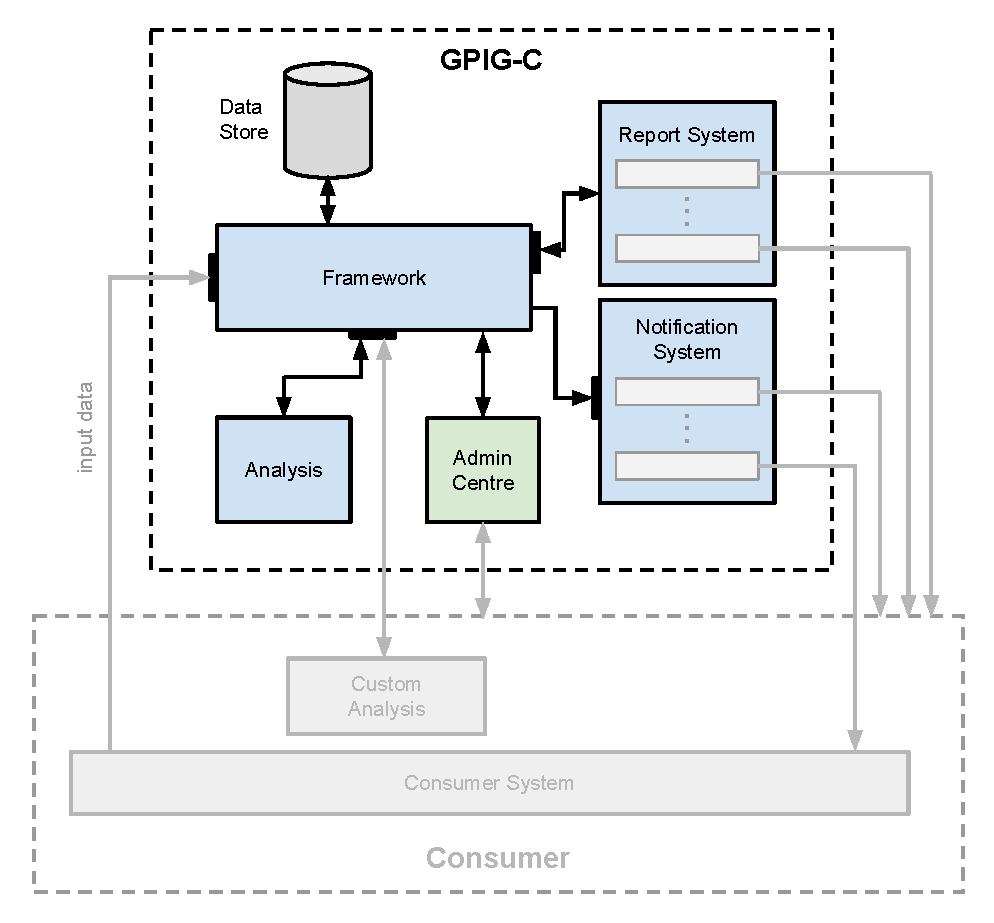
\includegraphics[width=0.75\textwidth]{system-architecture.pdf}
  \caption{System diagram}
\end{figure}

\section{Team organisation}

\subsection{Team members}

\subsection{Roles}


\section{Development plan}

\subsection{Software engineering methodology}

\subsection{Schedule}


\section{Risk register}


\section{Customer communication}


\end{document}
